\chapter{\emph{ATDlib}: A Library to Manage and Generate ATD}
\label{cha:atdlib}

This chapter presents \emph{ATDlib}, a reference implementation of the ATD
langauge described in Chapter~\ref{cha:atd} which implements parsing, automatic
generation and transformations of ATD. Section~\ref{sec:architecture} focuses on
the several tools provided in ATDlib and offers implementation details. Then,
Section~\ref{sec:atdlib_tour} shows an overview of the process of creating an
ATD from raw text data.

\section{Features and Architecture}
\label{sec:architecture}

The main goal behind ATDlib is to provide the necessary tooling in order to
support the implementation of ATD in organizations as a way of describing
business processes. This major goal can be split into the following
functionalities:


\begin{description}
  \item[Parsing and Representation of ATD]{ATD are stored as BRAT annotation
      files in \emph{standoff format}\cite{brat_standoff}. The standoff format
      is a text-based file that represents \emph{annotations} and
      \emph{relations} referencing a plain text file. Thus, an ATD will consist
      of a \texttt{Process.txt} with the textual description and a complementary
      \texttt{Process.ann} file with the annotations. ATDlib can parse this
      format and convert it to its internal schema, exposed in a public
      interface as shown in the UML diagram of Figure~\ref{fig:atdlib_uml}}
  \item[Automatic Annotation]{ATDlib can perform an initial annotation of a raw
      text in natural language. The goal is to perform the most accurate
      annotations possible. However, due to limitations in NLP, the annotations
      generated need to be reviewed by a human. Currently all annotation and
      relation types described in Section~\ref{sec:atd_semantics} are generated
      except the \emph{sequential}, \emph{exclusive} and \emph{parallel}
      relations, which must be manually annotated.}
  \item[Automatic Translation]{Several transformations are implemented for ATD
      in order to generate other process representations that interface with
      existing software. The goal is to establish ATD as a unique language for
      which any other representation can be automatically derived. These
      transformations can then be implemented as additional modules in ATDlib.
      Currently, the implemented transformations are to convert ATD into a
      FreeLing\cite{PadroS12} \emph{semantic graphs} and a \emph{behavioral
        profiles}\cite{smirnov2010business}}
    
\end{description}


ATDlib is structured as a single java library with several entry points,
corresponding to its different modules. Figure~\ref{fig:atdlib_architecture}
shows an overview of the different entry points, and their main functionalities.
The \texttt{brat\_parser} module is intended to be used as a library, and can be
used to read an annotation file into a more friendly format. The \texttt{text2atd}
entry point can be used as a standalone tool or as a library, and converts
textual descriptions into partially annotated ATD, which should then be checked
by a human using any compatible annotation tool, such as BRAT. Finally, the
\texttt{atd2fl} and \texttt{atd2bp} modules can be used as libraries to extract
a FreeLing semantic graph and a behavioral provile respectively. The inference
rules described in Section~\ref{sec:atd_reasoning} are applied during the
transformations. As mentioned in Section~\ref{sec:background_nlp4bpm}, the
semantic graph and the behavioral profiles can then be applied directly as input
data to the algorithms in the \emph{NLP4BPM} project.

\begin{figure}[htb]
  \centering
  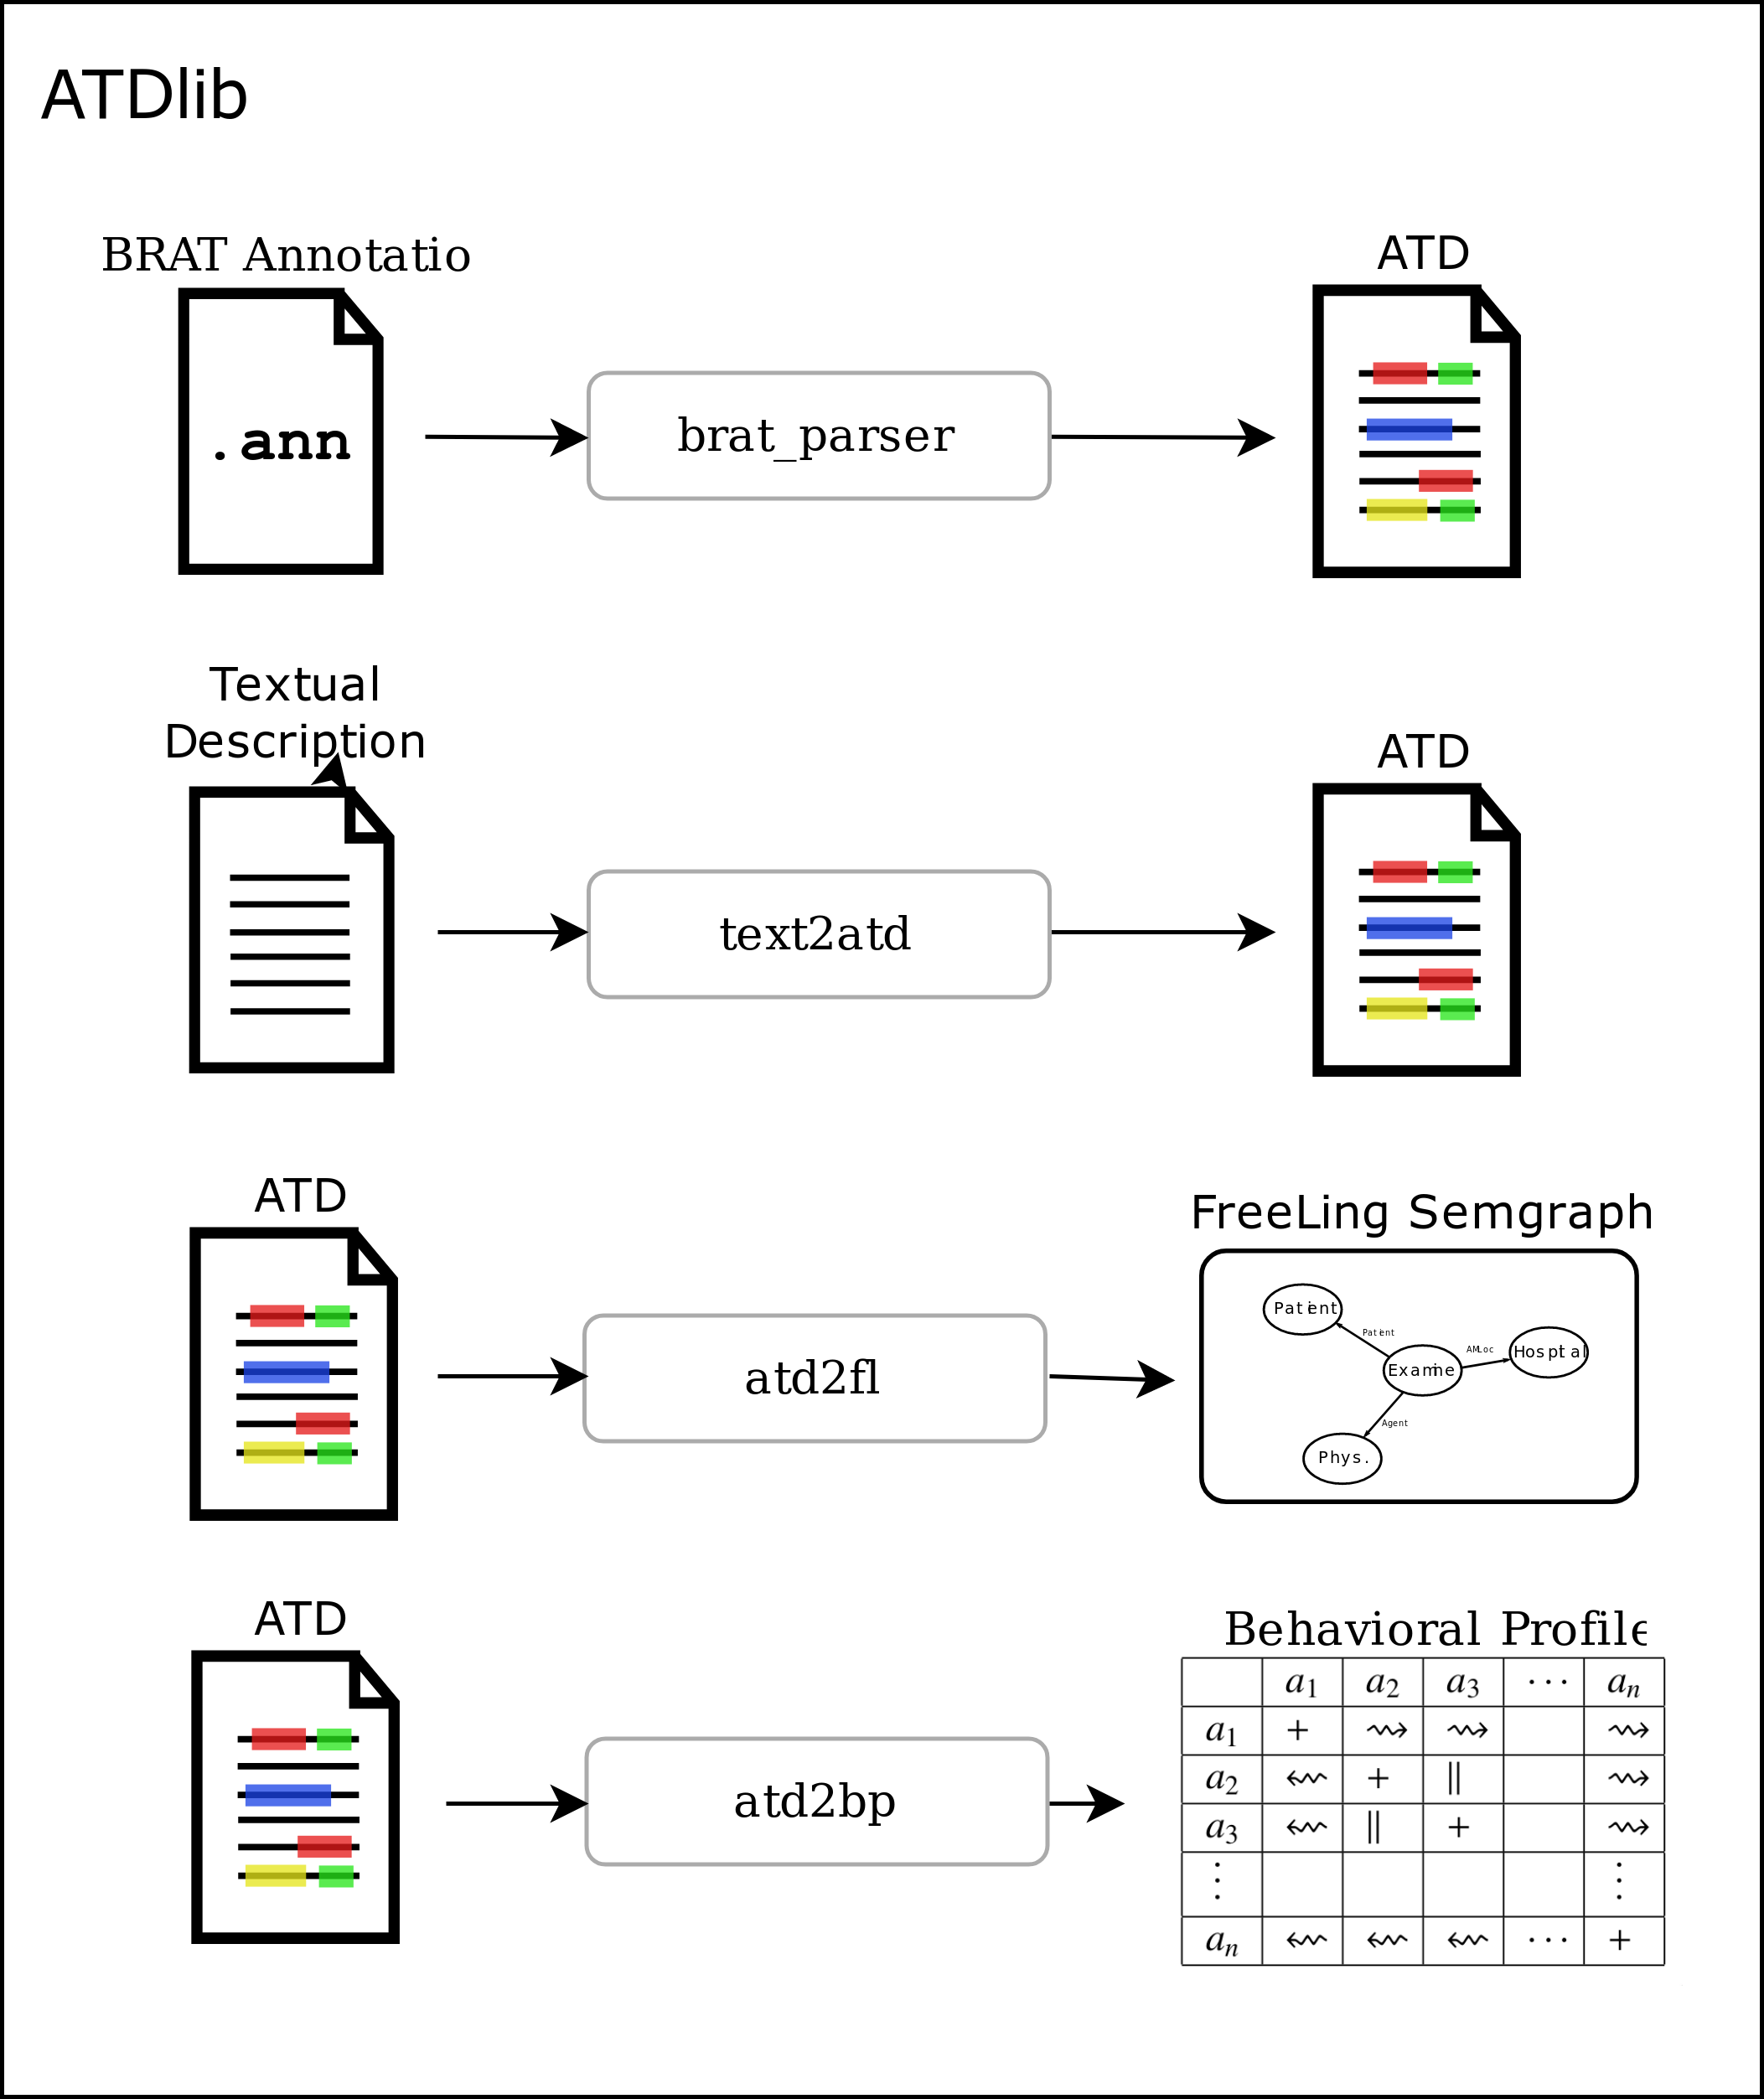
\includegraphics[width=0.75\textwidth]{figures/atdlib_arch}
  \caption{ATDlib feature overview}
  \label{fig:atdlib_architecture}
\end{figure}


\begin{figure}[htb]
  \centering
  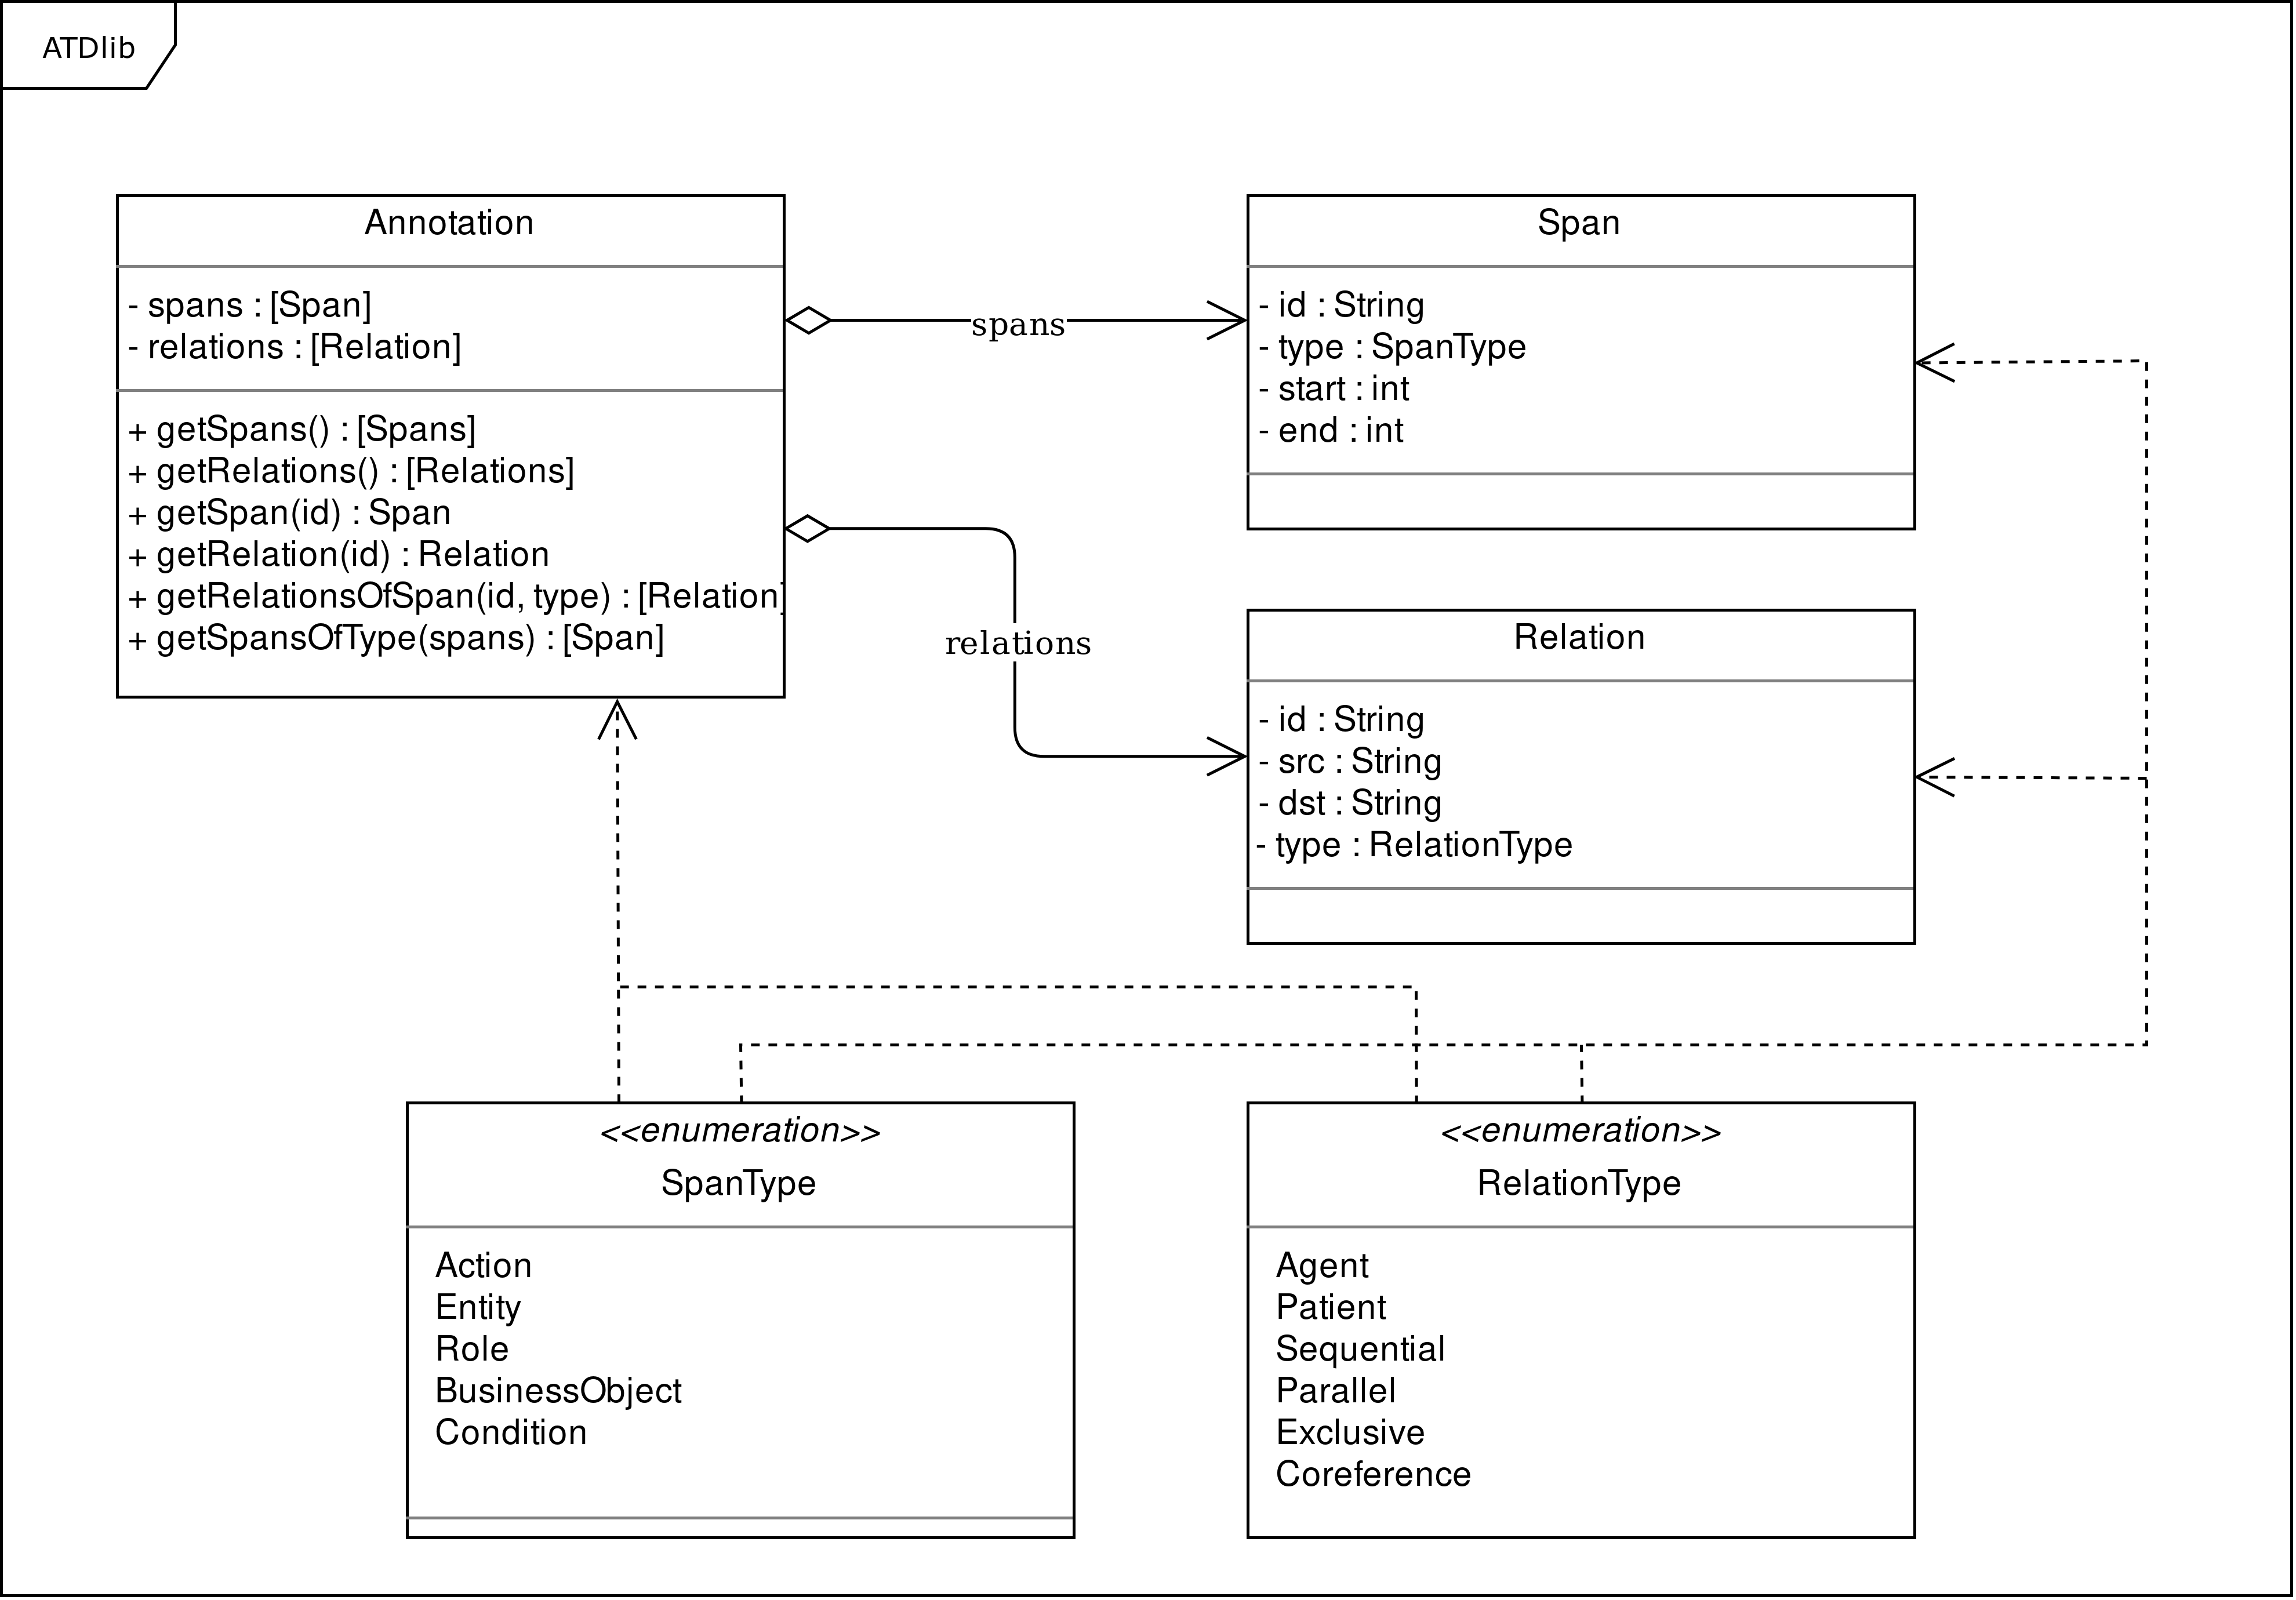
\includegraphics[width=\textwidth]{figures/atdlib_uml}
  \caption{UML diagram showing the public interface used for ATD representation}
  \label{fig:atdlib_uml}
\end{figure}

\todo{Explain ATD2FL algorithm!!!}


\section{Creating an ATD with \emph{ATDlib}}
\label{sec:atdlib_tour}

Figure~\ref{fig:atdlib_process} illustrates the steps that must be taken in
order to generate a full ATD with ATDlib. First, a human actor must describe
the business process using natural language, creating a \texttt{MyProcess.txt}
file. Next, the \texttt{text2atd} module is used in order to obtain an
annotation file, \texttt{MyProcess.ann}. The user can then inspect the generated
annotation using the BRAT web interface. Figure~\ref{fig:brat_example} (left)
shows an example of what the user will see in the screen at this point. The user
must then refine the annotation, usually this process consists of deleting the
irrelevant actions detected by ATDlib, as well as marking the control flow for
the final set of actions, resulting in an annotation file similar to the one
shown in Figure~\ref{fig:brat_example} (right). Finally, if necessary, ATDlib
can be used to generate other process model representations, such as a FreeLing
semantic graph using the \texttt{atd2fl} module.

\begin{figure}[htb]
  \centering
  \begin{minipage}{0.49\textwidth}
  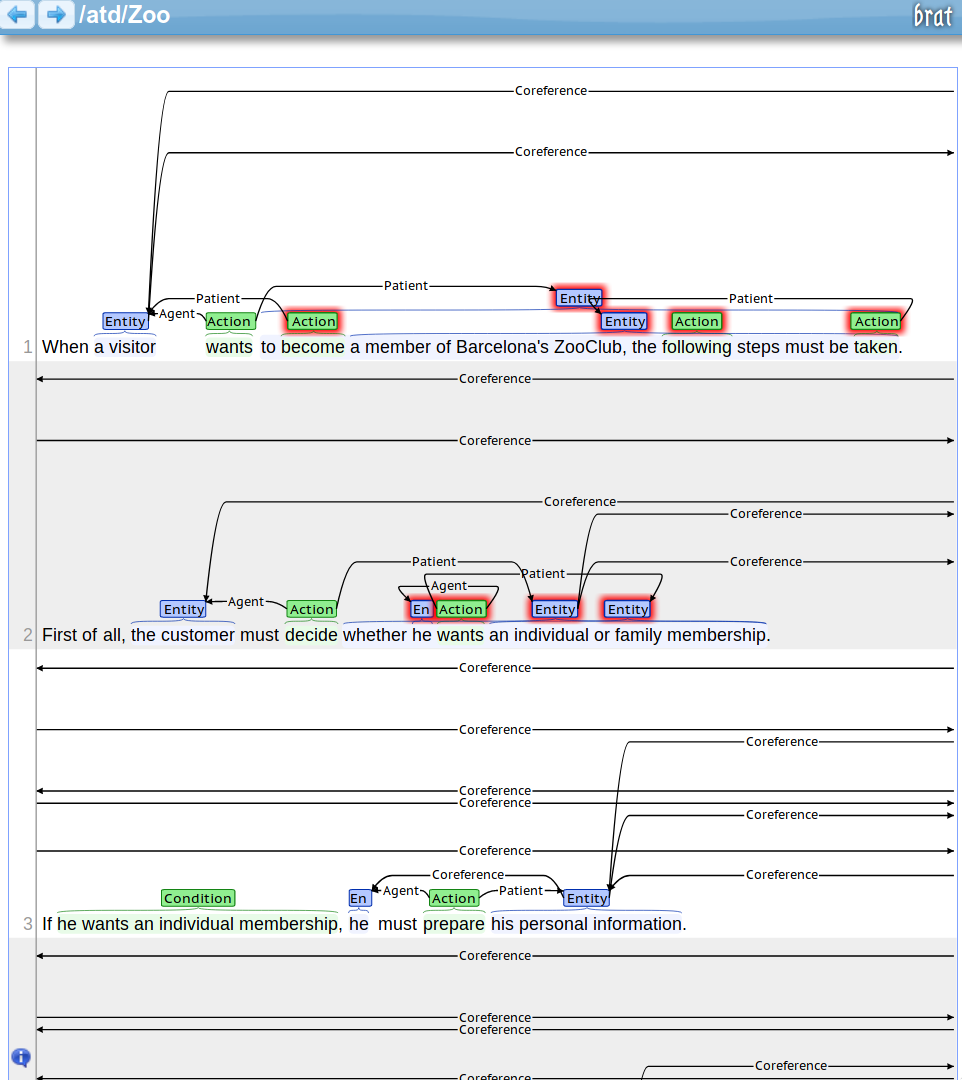
\includegraphics[width=\textwidth]{figures/ann_example_auto}
  \end{minipage}
  \begin{minipage}{0.49\textwidth}
  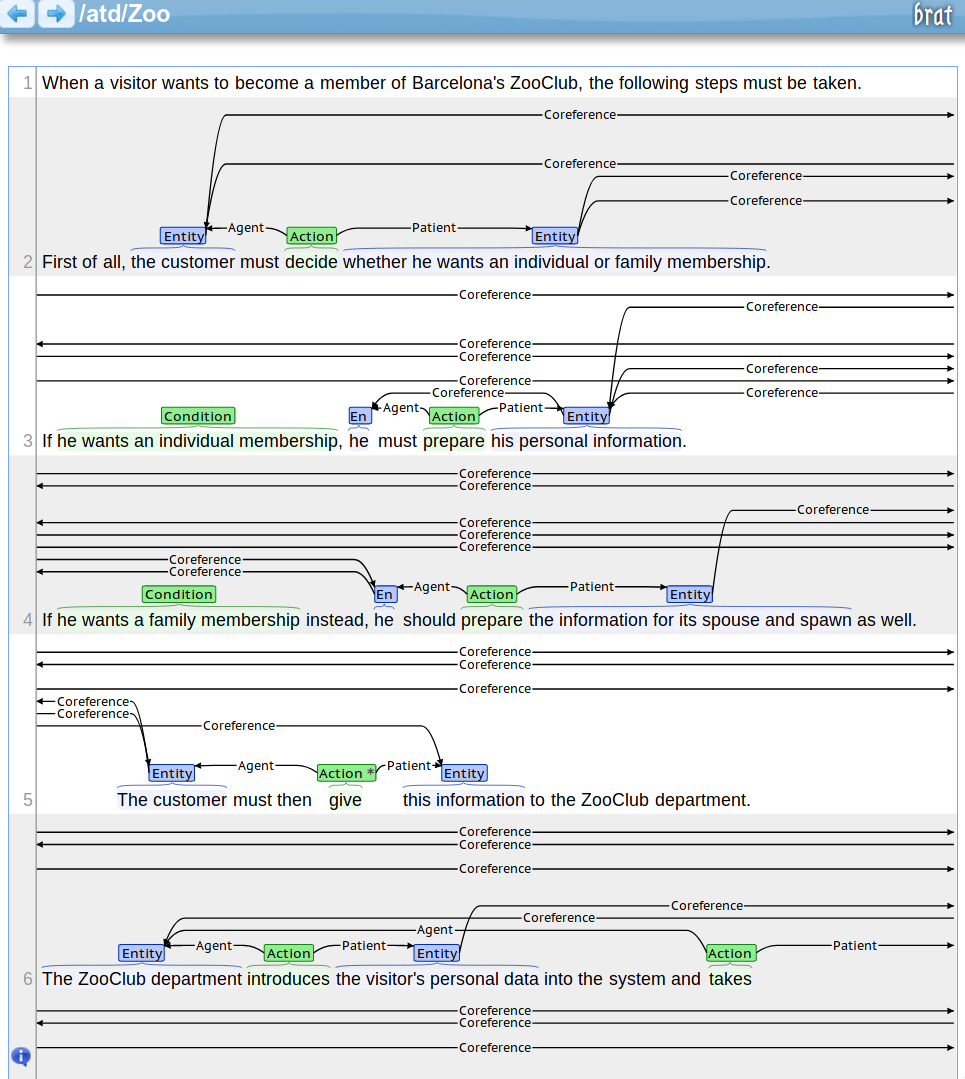
\includegraphics[width=\textwidth]{figures/ann_example_final}
  \end{minipage}
  \caption{The brat user interface: (left) An automatically generated
    ATD. (right) After the user performs a manual validation.}
  \label{fig:brat_example}
\end{figure}


\begin{figure}[htb]
  \centering
  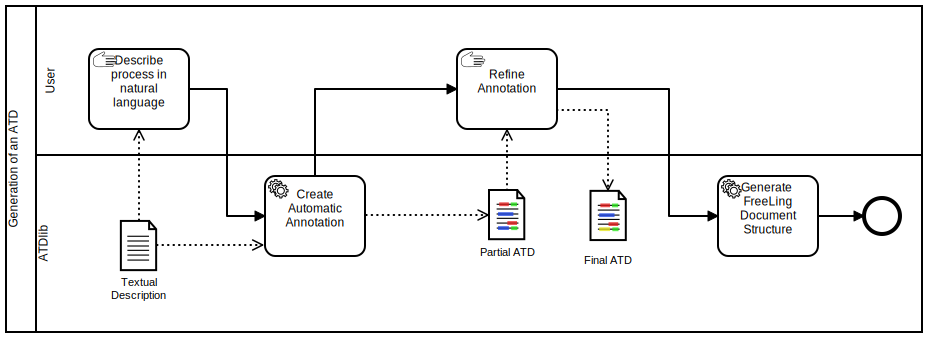
\includegraphics[width=\textwidth]{figures/atdlib_bpmn}
  \caption{Workflow of the creation of an ATD using ATDlib}
  \label{fig:atdlib_process}
\end{figure}

